\documentclass[dvipdfmx]{jlreq}
\usepackage{keyval}
\usepackage{physics}
\usepackage{fancybox}
\usepackage{ascmac}
\usepackage{tcolorbox}
\usepackage{amsmath}
\usepackage{mathrsfs}
\usepackage[utf8]{inputenc}
\usepackage{graphicx}
\usepackage{subcaption}
\usepackage{hyperref}
\usepackage{bookmark}
\usepackage{color}
\usepackage[version=4]{mhchem}
\usepackage{float}
\usepackage{braket}
\usepackage{mathtools}
\usepackage[top=25.4truemm,bottom=25.4truemm,left=19.05truemm,right=19.05truemm]{geometry}
\usepackage[stable]{footmisc}
\usepackage{hhline}
\usepackage{rotating}
\usepackage{url}

\geometry{left=20mm,right=20mm,top=25mm,bottom=25mm}
\title{宇宙物理学 レポート課題}
\author{BHB26052 河村太星}
\date{\today}

\begin{document}

\maketitle

現代の標準宇宙論($\Lambda$CDMモデル)において、宇宙の膨張はロバートソン・ウォーカー(Robertson-Walker)計量によって記述される。本レポートでは、平坦な宇宙(空間曲率$\Omega_{\mathrm{k},0}=0$)を仮定し、宇宙論的赤方偏移$z$と、共動距離$D_{\mathrm{C}}$、光度距離$D_{\mathrm{L}}$、角度直径距離$D_{\mathrm{A}}$、およびルックバックタイム$t_{\mathrm{L}}$の関係式を導出・整理する。また、Planck(2018)の観測に基づく宇宙論パラメーターを用いて各物理量を数値計算し、その挙動をグラフによって視覚化する。

\section{基礎方程式と宇宙論パラメーター}
平坦なフリードマン・ルメートル・ロバートソン・ウォーカー(FLRW)宇宙における時空の線素$ds$は次式で与えられる。
\begin{equation}
    ds^2 = -c^2 dt^2 + a(t)^2 \left[ dr^2 + r^2 (d\theta^2 + \sin^2\theta d\phi^2) \right]
\end{equation}
ここで、$a(t)$は現在の値を$a(t_0)=1$に規格化したスケール因子であり、赤方偏移$z$との間には次の関係がある。
\begin{equation}
    1 + z = \frac{1}{a(t)}
\end{equation}
任意の赤方偏移$z$におけるハッブル関数$H(z)$は、物質の密度パラメーター$\Omega_{\mathrm{m},0}$、ダークエネルギー(宇宙項)の密度パラメーター$\Omega_{\Lambda,0}$を用いて以下のように表される。
\begin{equation}
    H(z) = H_0 E(z) = H_0 \sqrt{\Omega_{\mathrm{m},0}(1+z)^3 + \Omega_{\Lambda,0}}
\end{equation}
今回は、Planck(2018)の観測成果に基づき、以下のパラメーターを採用する。
\begin{itemize}
    \item ハッブル定数: $H_0 = 67.4 \ \mathrm{km/s/Mpc}$
    \item 物質密度パラメータ: $\Omega_{\mathrm{m},0} = 0.315$
    \item ダークエネルギー密度パラメータ: $\Omega_{\Lambda,0} = 0.685$
    \item ハッブル距離: $D_{\mathrm{H}} = \frac{c}{H_0} \approx 4448 \ \mathrm{Mpc}$
    \item ハッブル時間: $t_{\mathrm{H}} = \frac{1}{H_0} \approx 14.5 \ \mathrm{Gyr}$
\end{itemize}

\section{共動距離(Comoving Distance: $D_{\mathrm{C}}$)の導出}
共動距離は、宇宙の膨張に伴って伸び縮みする座標系において定義される距離である。天体から地球に向かってまっすぐ($d\theta = d\phi = 0$)進む光($ds^2 = 0$)を考えると、次式が成り立つ。
\begin{equation}
    0 = -c^2 dt^2 + a(t)^2 dr^2 \implies dr = \frac{c dt}{a(t)}
\end{equation}
過去の時刻$t$に天体を出発した光が現在$t_0$に到達するまでの共動座標の差$r$は、これを積分することで得られる。時間微分と赤方偏移微分の関係式$dt = -\frac{dz}{(1+z)H(z)}$および$a(t) = (1+z)^{-1}$を用いて変数変換を行うと、共動距離$D_{\mathrm{C}} \equiv r$は以下のように導かれる。
\begin{equation}
    D_{\mathrm{C}}(z) = \int_{t}^{t_0} \frac{c dt'}{a(t')} = \int_{0}^{z} \frac{c dz'}{H(z')} = D_{\mathrm{H}} \int_{0}^{z} \frac{dz'}{E(z')}
\end{equation}

\section{光度距離(Luminosity Distance: $D_{\mathrm{L}}$)の導出}
天体の絶対光度$L$と地球で観測される見かけのフラックス$F$の間に、静的な空間と同様の逆二乗則$F = \frac{L}{4\pi D_{\mathrm{L}}^2}$が成り立つように定義された距離である。膨張宇宙においては、距離$D_{\mathrm{C}}$による幾何学的な広がりに加え、以下の2つの効果によってエネルギーが減少する。
\begin{enumerate}
    \item 膨張による光子の波長の伸び(赤方偏移)に伴い、光子1個あたりのエネルギーが$\frac{1}{1+z}$倍になる。
    \item 時間の遅れ(膨張空間の通過)により、光子の到着時間間隔が$(1+z)$倍に伸び、単位時間あたりの個数が$\frac{1}{1+z}$倍になる。
\end{enumerate}
これらにより、観測されるフラックスは$F = \frac{L}{4\pi D_{\mathrm{C}}^2 (1+z)^2}$となり、定義式と比較することで次式が得られる。
\begin{equation}
    D_{\mathrm{L}}(z) = (1+z)D_{\mathrm{C}}(z)
\end{equation}

\section{角度直径距離(Angular Diameter Distance: $D_{\mathrm{A}}$)の導出}
天体の固有の直径(実際の大きさ)$D$と、その見かけの角直径$\theta$の間に、ユークリッド空間的な関係$\theta = \frac{D}{D_{\mathrm{A}}}$が成り立つように定義された距離である。光が天体を出発した過去の時刻$t$における時空の長さ(固有長)$D$は、計量の空間成分より次のように表される。
\begin{equation}
    D = a(t) \cdot r \cdot \theta = \frac{D_{\mathrm{C}}}{1+z} \theta \implies \theta = \frac{D}{D_{\mathrm{C}}/(1+z)}
\end{equation}
これにより、角度直径距離$D_{\mathrm{A}}$は以下のように導かれる。
\begin{equation}
    D_{\mathrm{A}}(z) = \frac{D_{\mathrm{C}}(z)}{1+z} = \frac{D_{\mathrm{L}}(z)}{(1+z)^2}
\end{equation}

\section{ルックバックタイム(Look-back Time: $t_{\mathrm{L}}$)の導出}
赤方偏移$z$にある天体から放たれた光が、現在地球に到達するまでに経過した時間である。
\begin{equation}
    t_{\mathrm{L}}(z) = \int_{t}^{t_0} dt' = \int_{0}^{z} \frac{dz'}{(1+z')H(z')} = t_{\mathrm{H}} \int_{0}^{z} \frac{dz'}{(1+z')E(z')}
\end{equation}

\section{数値計算とグラフ化}
上述の関係式に基づき、Pythonを用いて$z=0$から$z=10$までの範囲を数値計算した。計算結果を図1と図2に示す。
\begin{figure}[htbp]
    \centering
    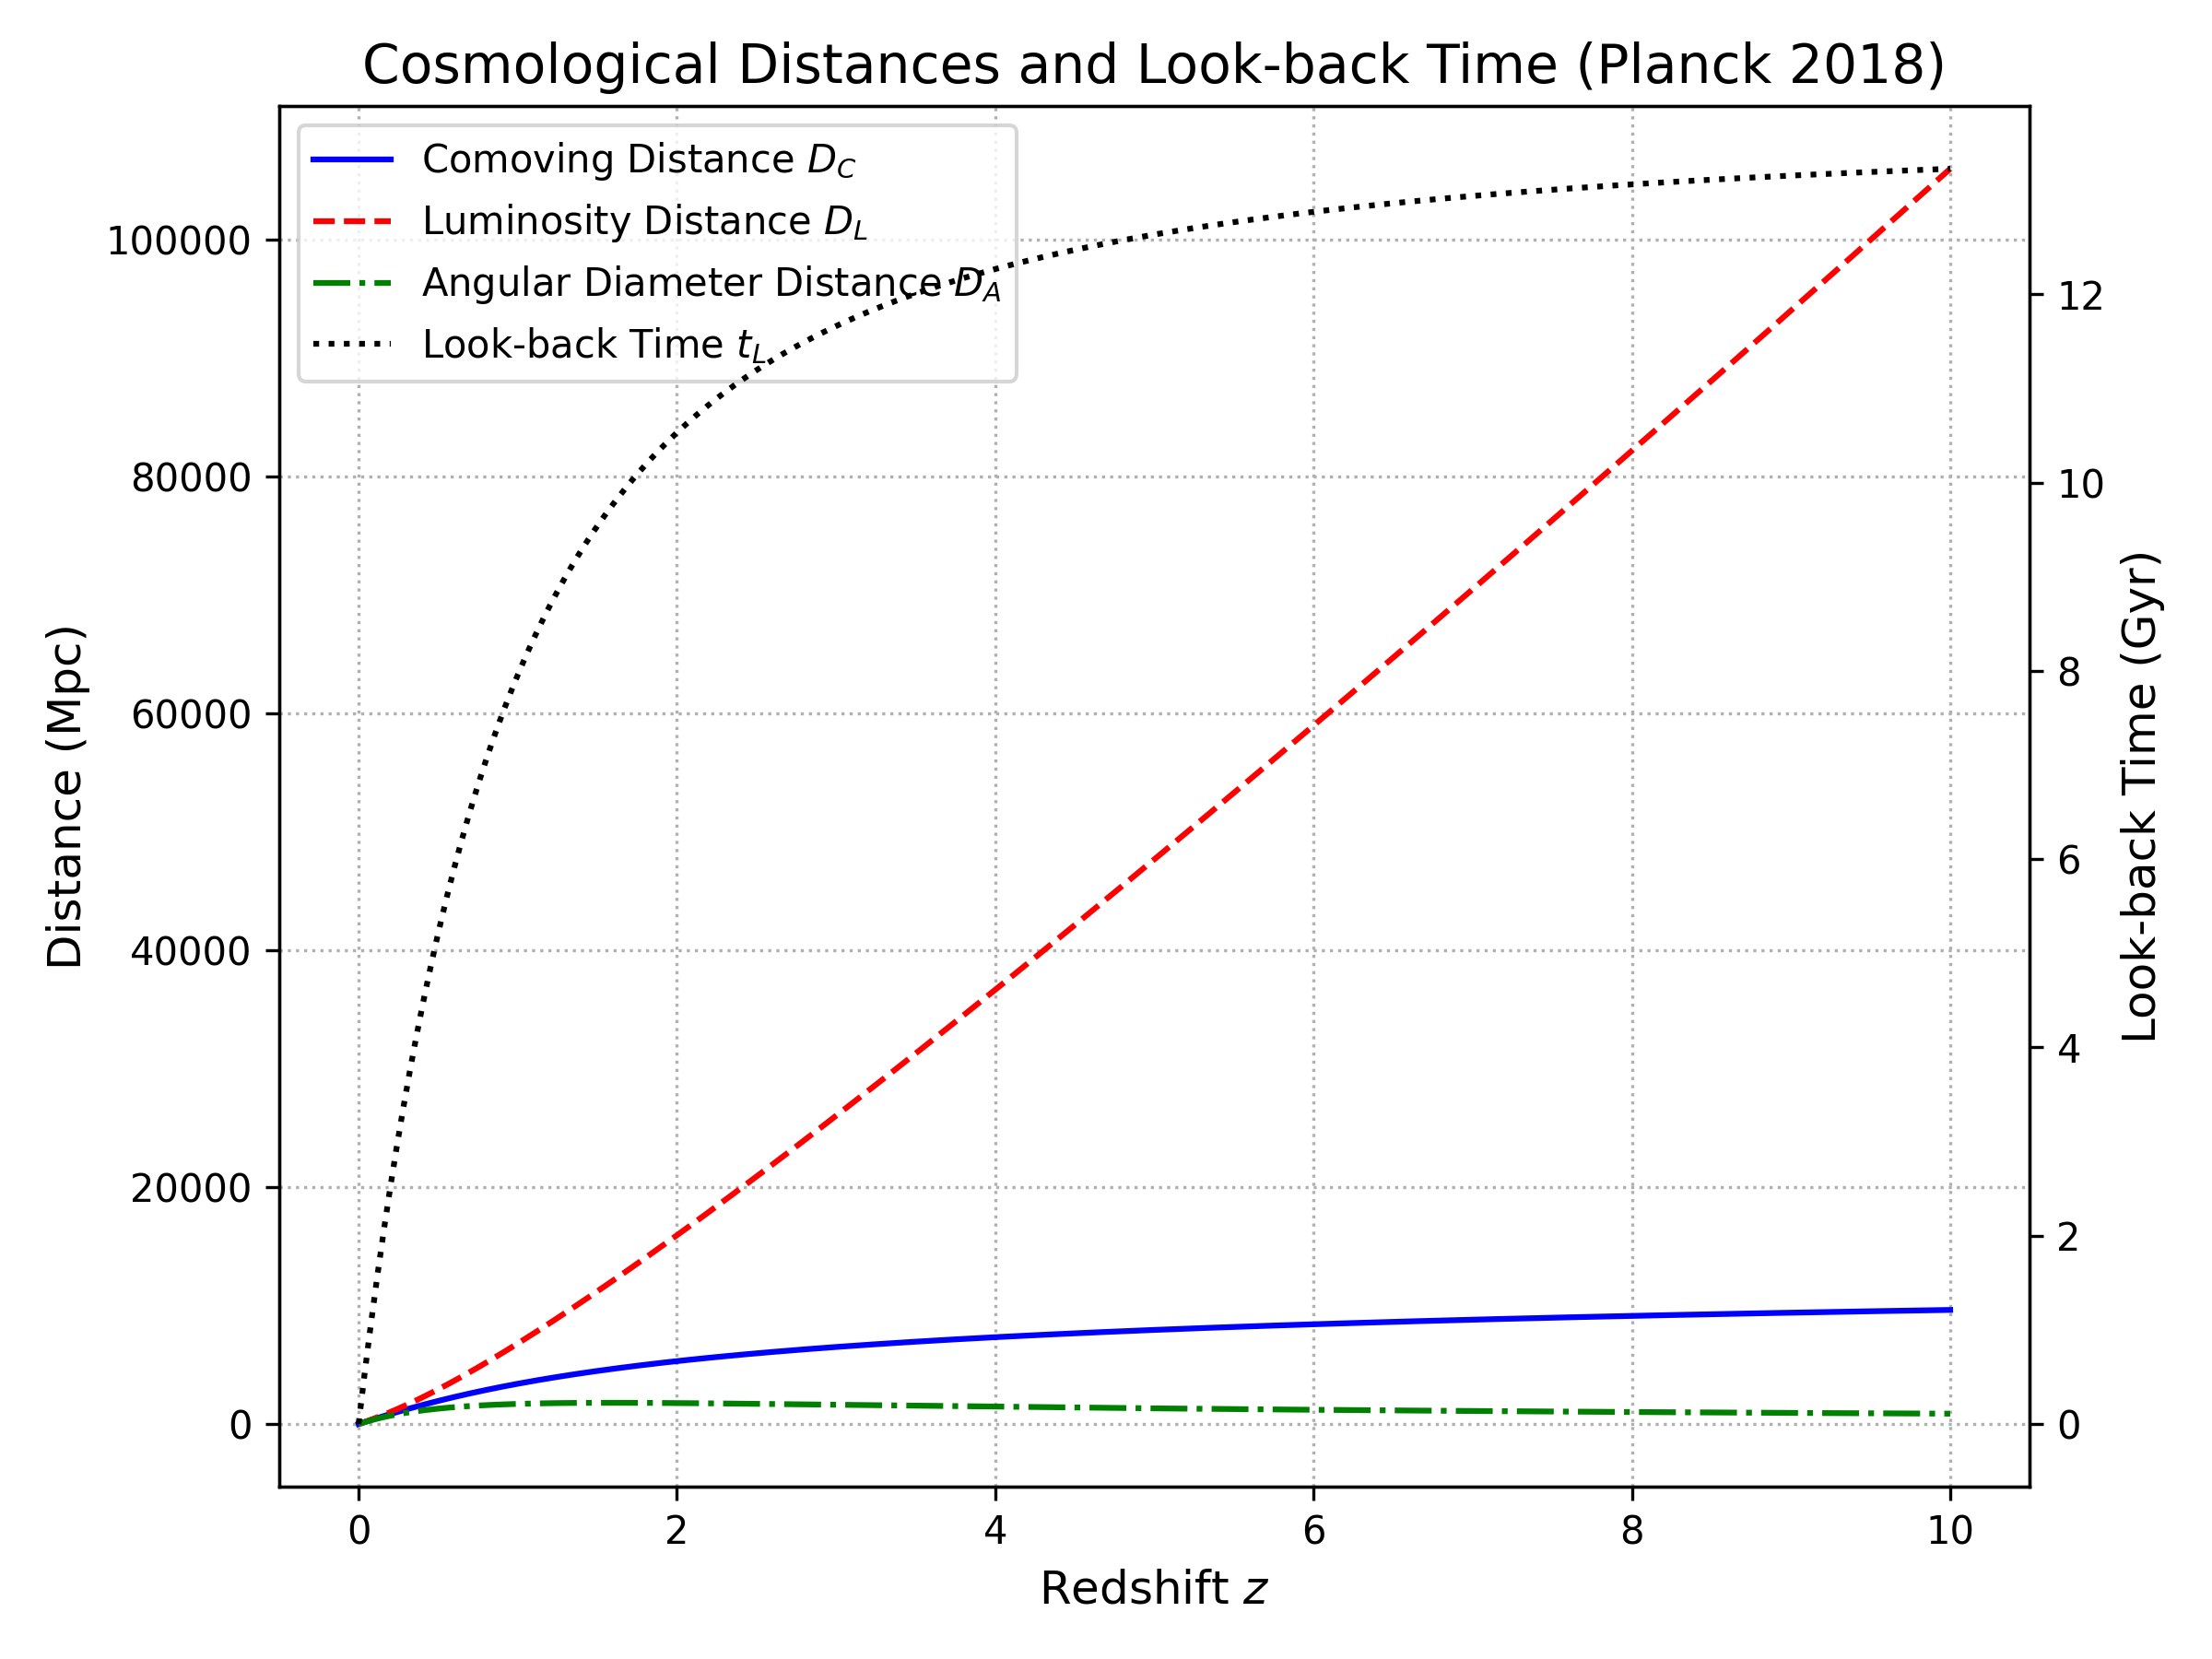
\includegraphics[width=0.6\textwidth]{cosmology_plot.png}
    \caption{赤方偏移$z$に対する各種宇宙論的距離(左軸)およびルックバックタイム(右軸)の依存性}
\end{figure}
\begin{figure}[htbp]
    \centering
    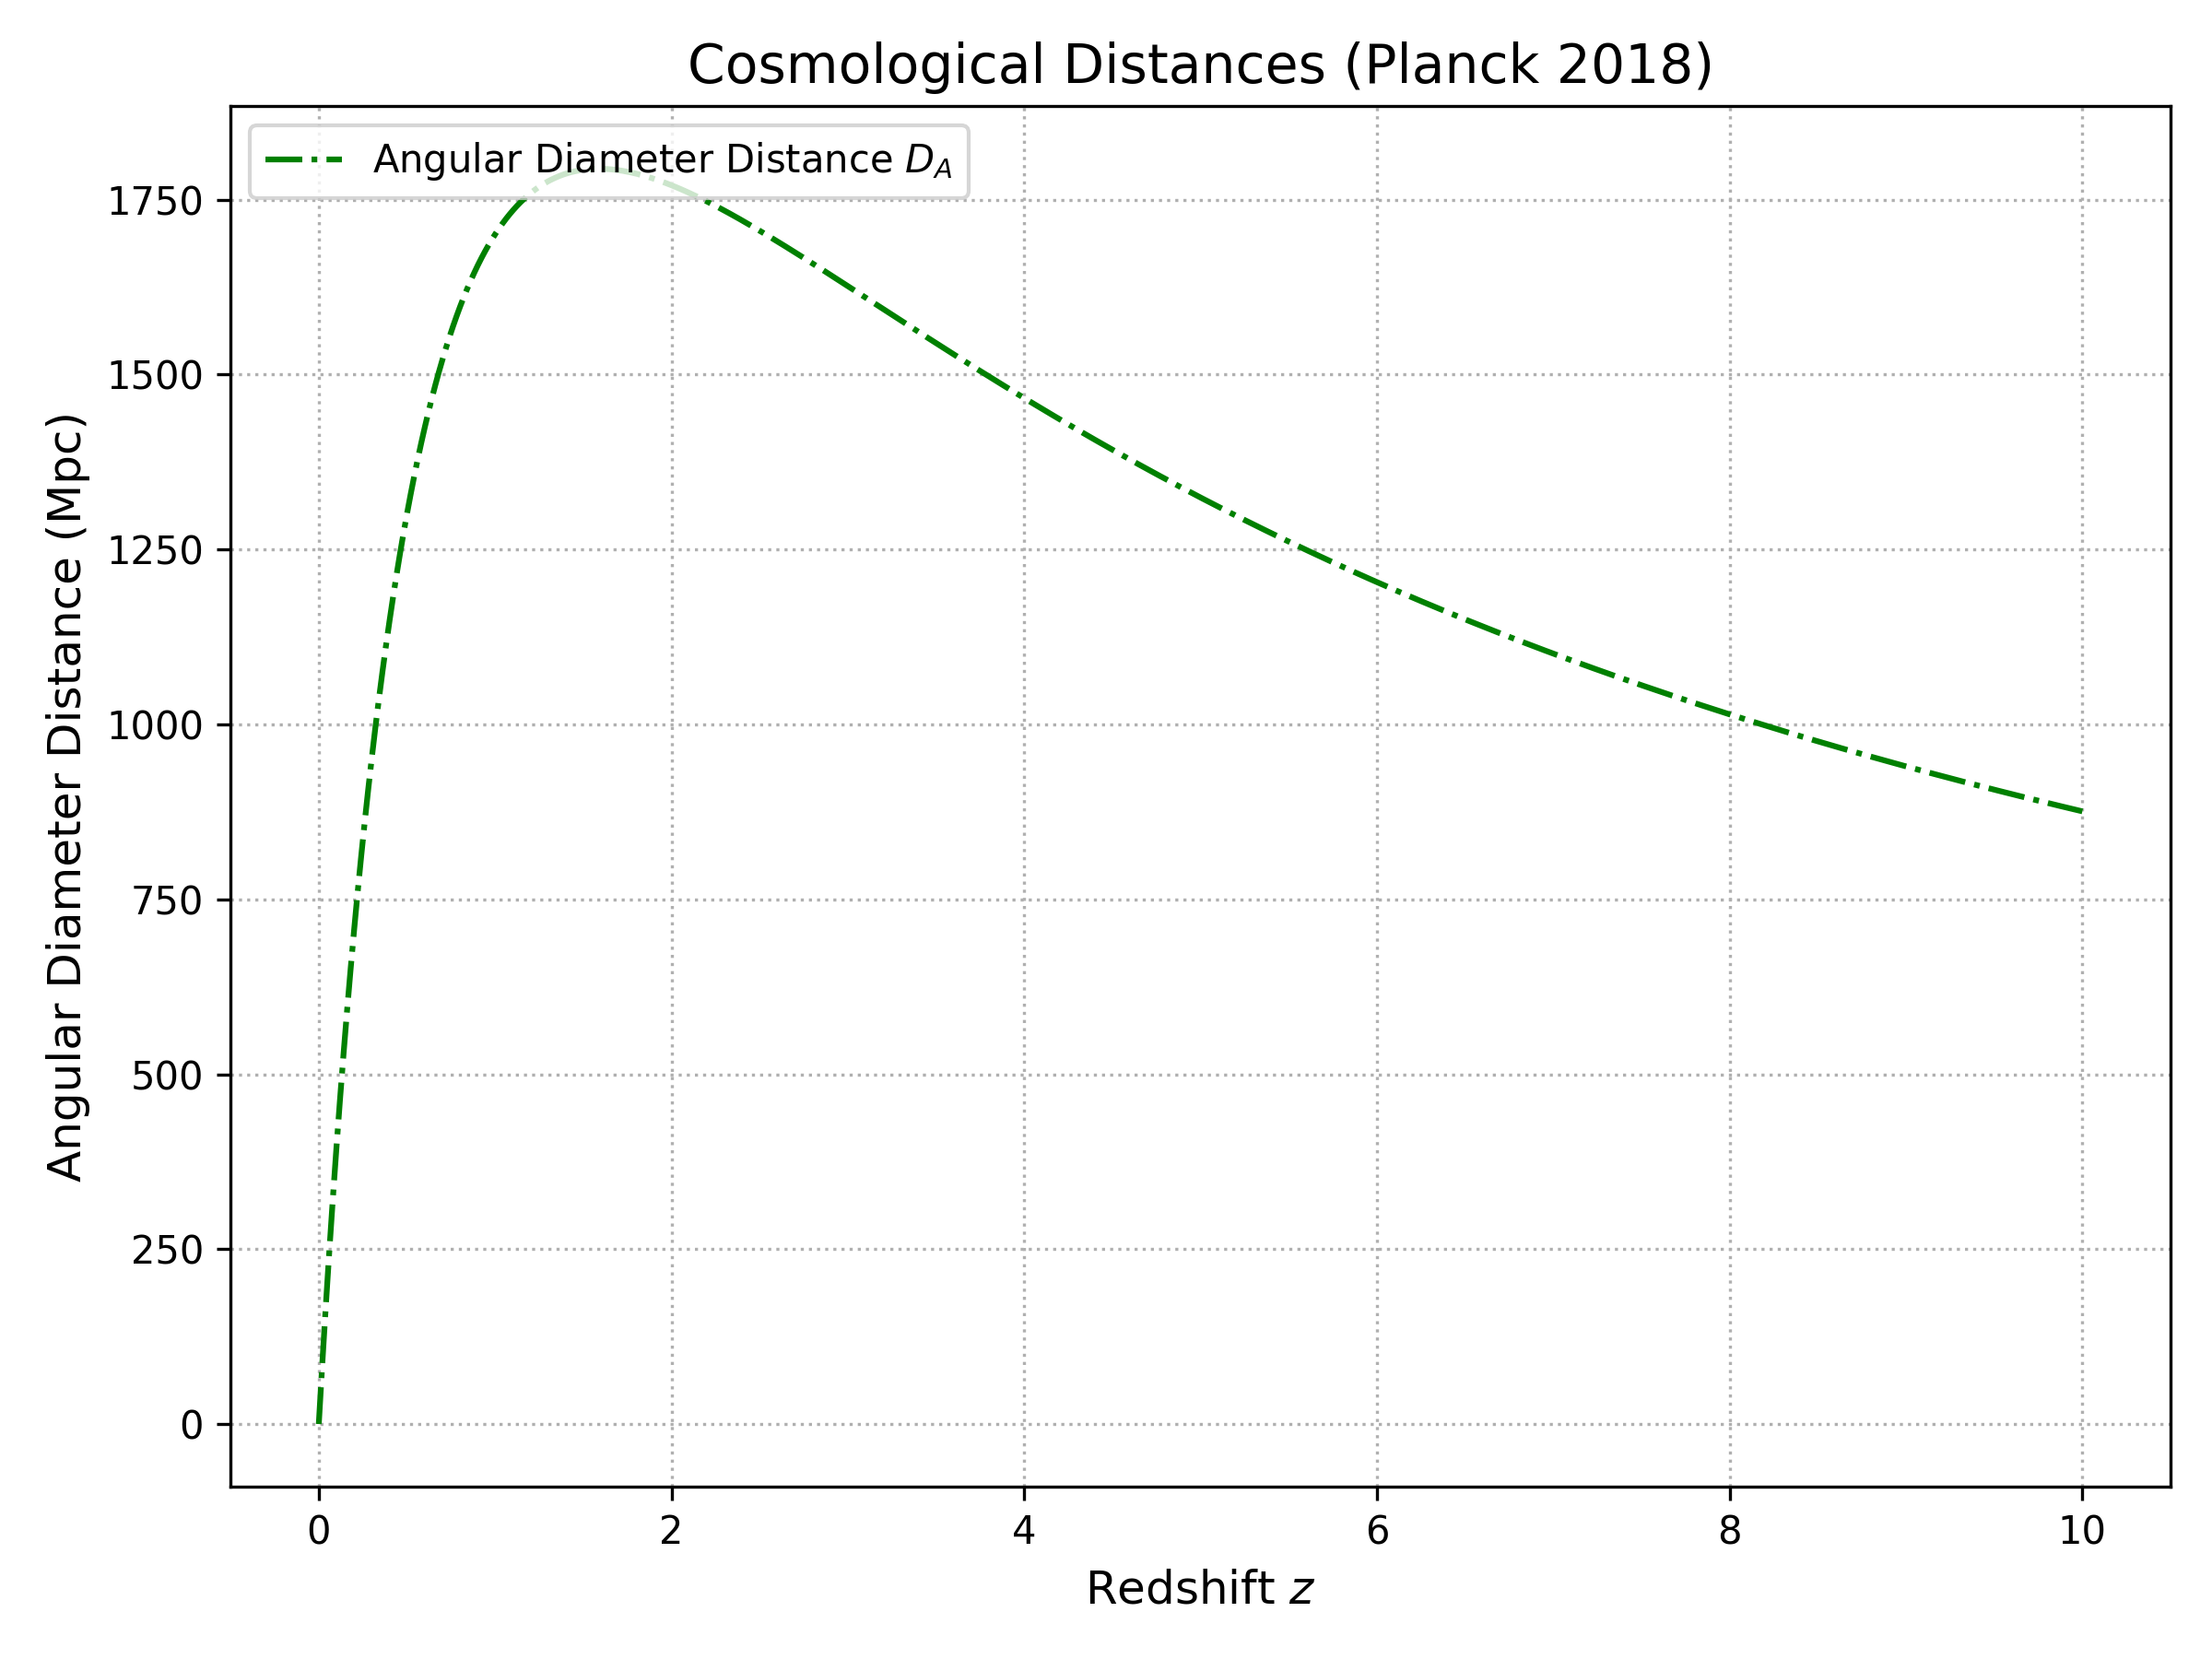
\includegraphics[width=0.6\textwidth]{cosmology_plot_angular.png}
    \caption{赤方偏移$z$に対する角度直径距離の依存性}
\end{figure}

\section{考察}
図1と図2から以下の特徴が読み取れる。
\begin{itemize}
    \item 光度距離$D_{\mathrm{L}}$の挙動: $(1+z)$の寄与により高赤方偏移ほど急激に増大する。これは、遠方の天体が宇宙膨張によって急速に暗く観測される物理背景を明確に示している。
    \item 角度直径距離$D_{\mathrm{A}}$の極大値: $z \approx 1.5$付近で極大値を迎え、それ以上の遠方では逆に天体が大きく(角直径が大きく)見えるという奇妙な現象が生じる。これは、光が放たれた当時の宇宙そのものが現在より小さく、天体と地球の物理的距離が近かったためである。
    \item ルックバックタイム$t_{\mathrm{L}}$の飽和: $z \to \infty$において、宇宙年齢(約138億年)に対応する有限の値に収束していく様子が見て取れる。
\end{itemize}

\begin{thebibliography}{9}
\bibitem{planck2018} Planck Collaboration, et al., ``Planck 2018 results. VI. Cosmological parameters,'' (2020).
\bibitem{hogg1999} Hogg, D. W., ``Distance measures in cosmology,'' (1999).
\end{thebibliography}

\end{document}